% Appendix Template

\chapter{Instrucciones} % Main appendix title

\label{App_Inst} % Change X to a consecutive letter; for referencing this appendix elsewhere, use \ref{AppendixX}

A continuación se presentan una serie de capturas de pantalla donde se presentan las instrucciones proporcionadas a los participantes en los Experimentos realizados.\\

\begin{figure}[th]
\centering
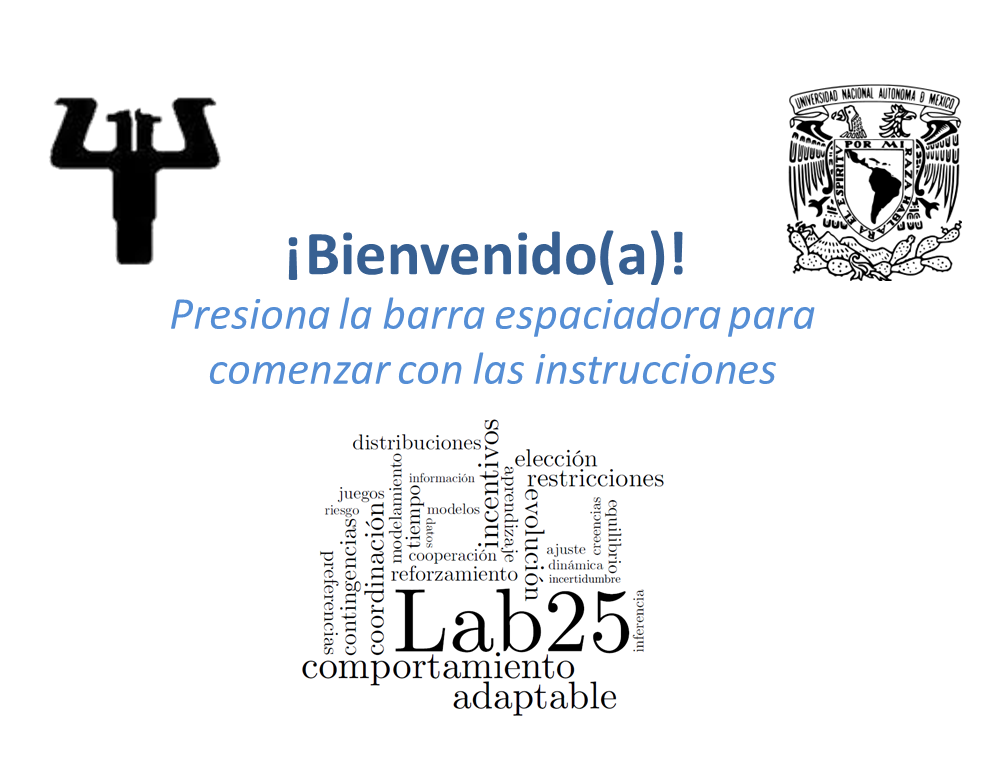
\includegraphics[width=0.95\textwidth]{Figures/Inst_Bienvenido} 
\decoRule
\caption[Pantalla de Bienvenida]{Una vez que los participantes ingresaban al espacio designado para realizar los experimentos, se encontraban con esta pantalla de bienvenida. El tiempo de realización del experimento comenzaba a registrarse a partir de que el participante diese \textit{Enter}.}
\label{fig:csv}
\end{figure}

\begin{figure}[th]
\centering
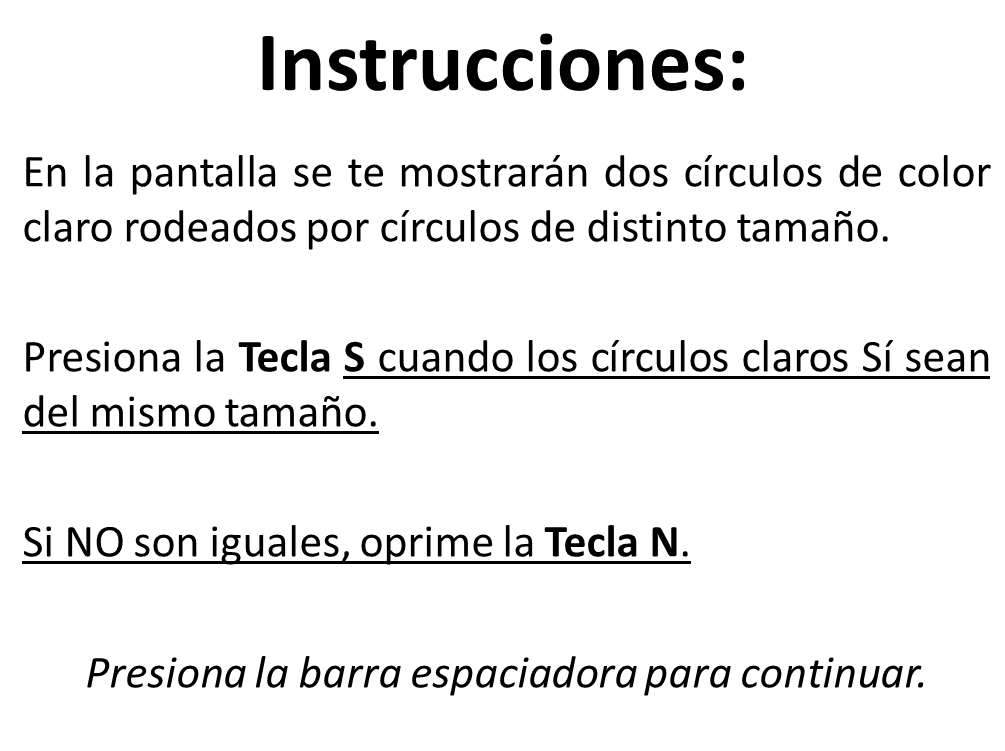
\includegraphics[width=0.75\textwidth]{Figures/Inst_1} 
\decoRule
\caption[Instrucciones principales]{La primera pantalla de instrucciones presentaba la tarea de detección central: identificar los ensayos donde dos círculos presentados en pantalla fueran del mismo tamaño.}
\label{fig:csv}
\end{figure}

\begin{figure}[th]
\centering
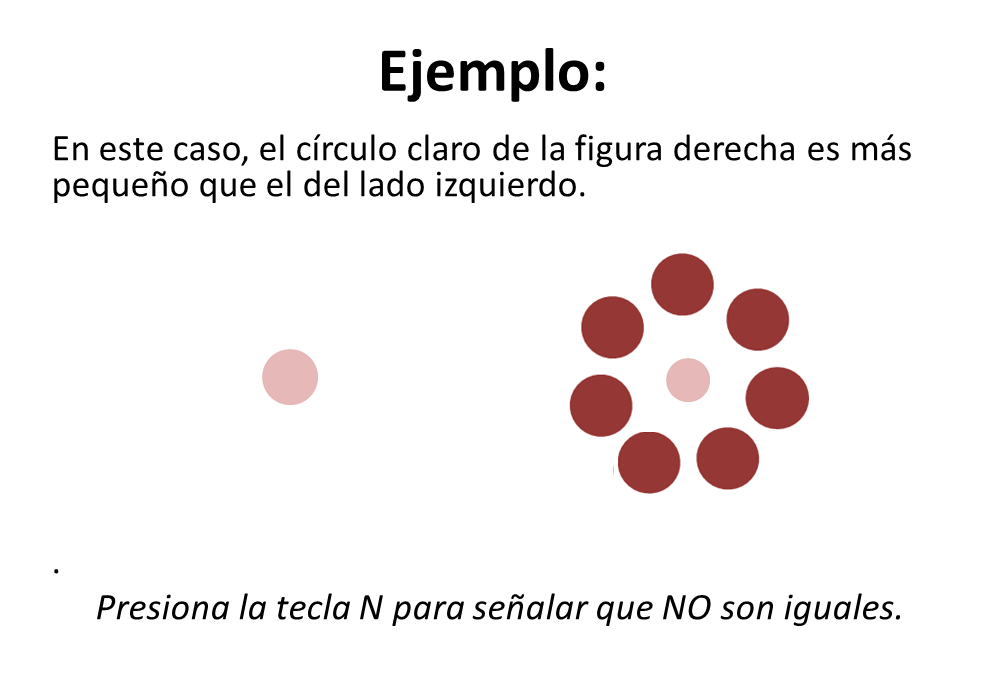
\includegraphics[width=0.85\textwidth]{Figures/Inst_Ex} 
\decoRule
\caption[Presentación de ejemplo]{Posteriormente, se les presentaba un ejemplo sobre cómo se verían los estímulos a comparar durante su participación y cuál es la tarea a la que se esperaba respondieran.}
\label{fig:csv}
\end{figure}

\begin{figure}[th]
\centering
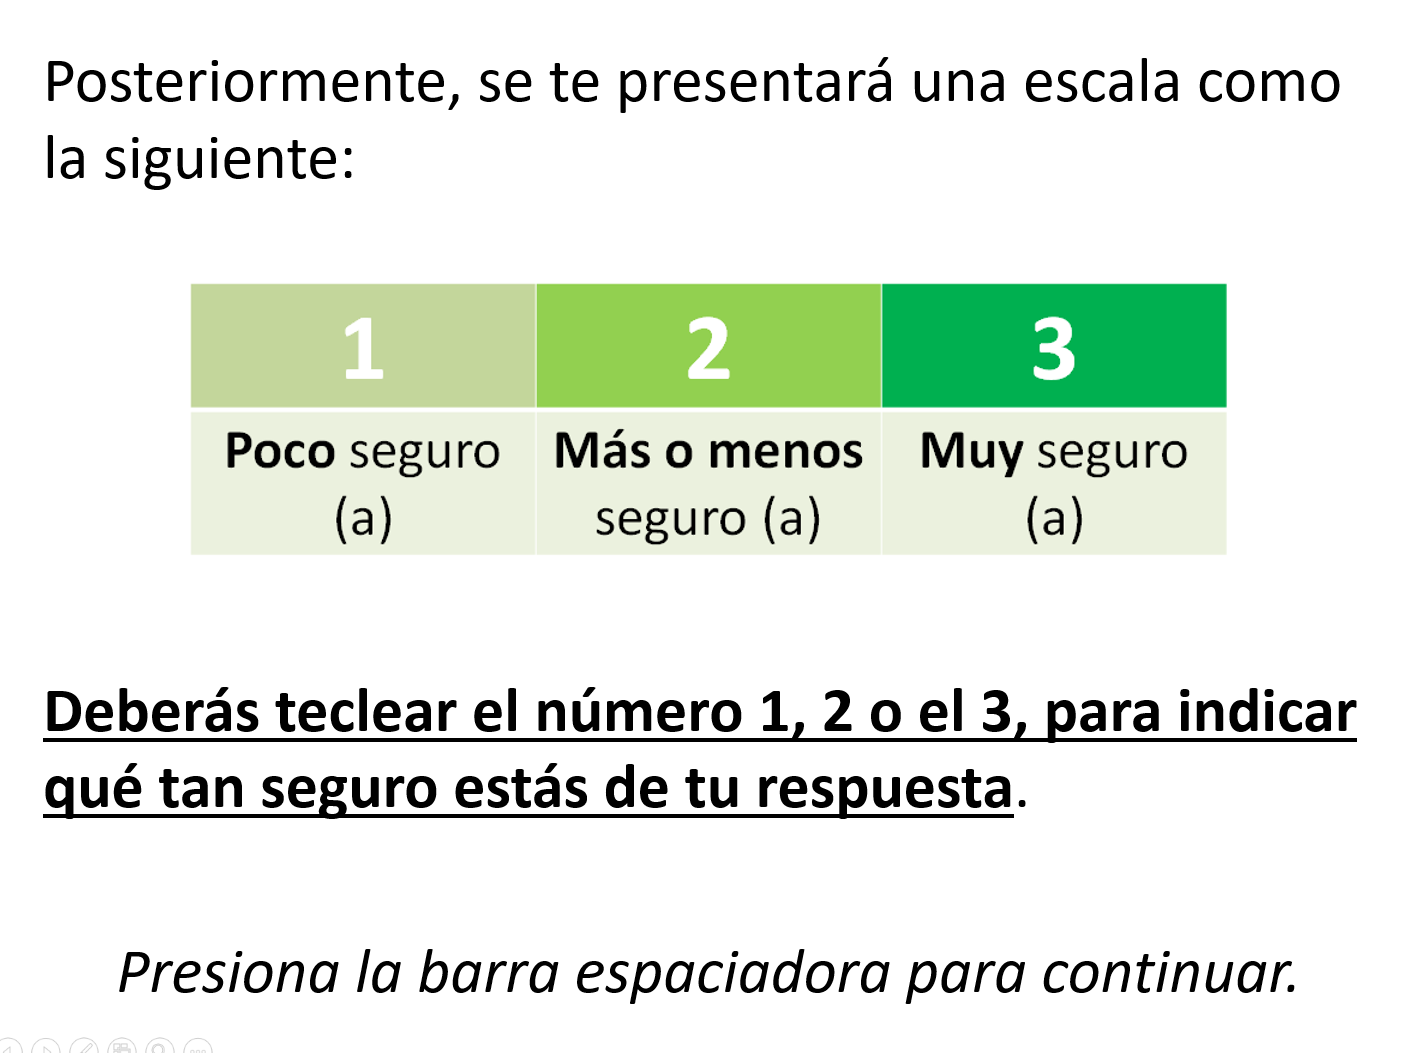
\includegraphics[width=0.75\textwidth]{Figures/Inst_Regla} 
\decoRule
\caption[Presentación de la tarea con Escala de Confianza]{Después, se les indicaba que deberían juzgar cuánta confianza tenían en la respuesta emitida al mostrarse en pantalla la Escala de Confianza.}
\label{fig:csv}
\end{figure}

\begin{figure}[th]
\centering
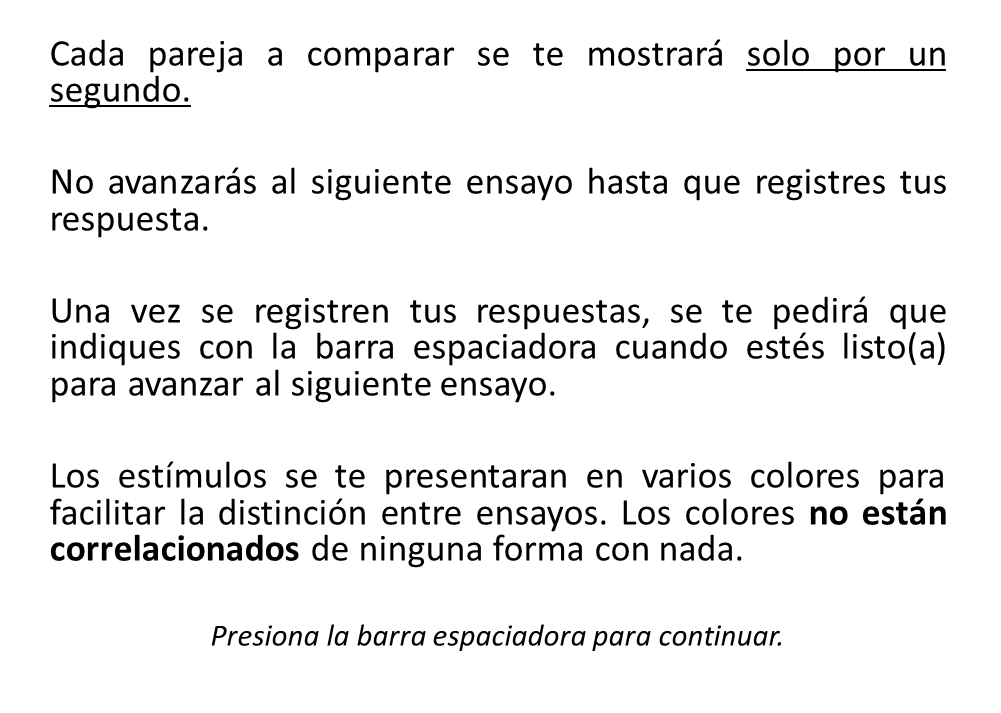
\includegraphics[width=0.85\textwidth]{Figures/Inst_3} 
\decoRule
\caption[Precisiones sobre la evaluación de la ejecución]{Finalmente, se hacían del conocimiento del participante algunas precisiones sobre la forma en que sería evaluada su ejecución, solicitándoles que fueran tan rápidos como pudieran y que hicieran caso omiso del color en que se le presentaban las figuras.}
\label{fig:csv}
\end{figure}

\begin{figure}[th]
\centering
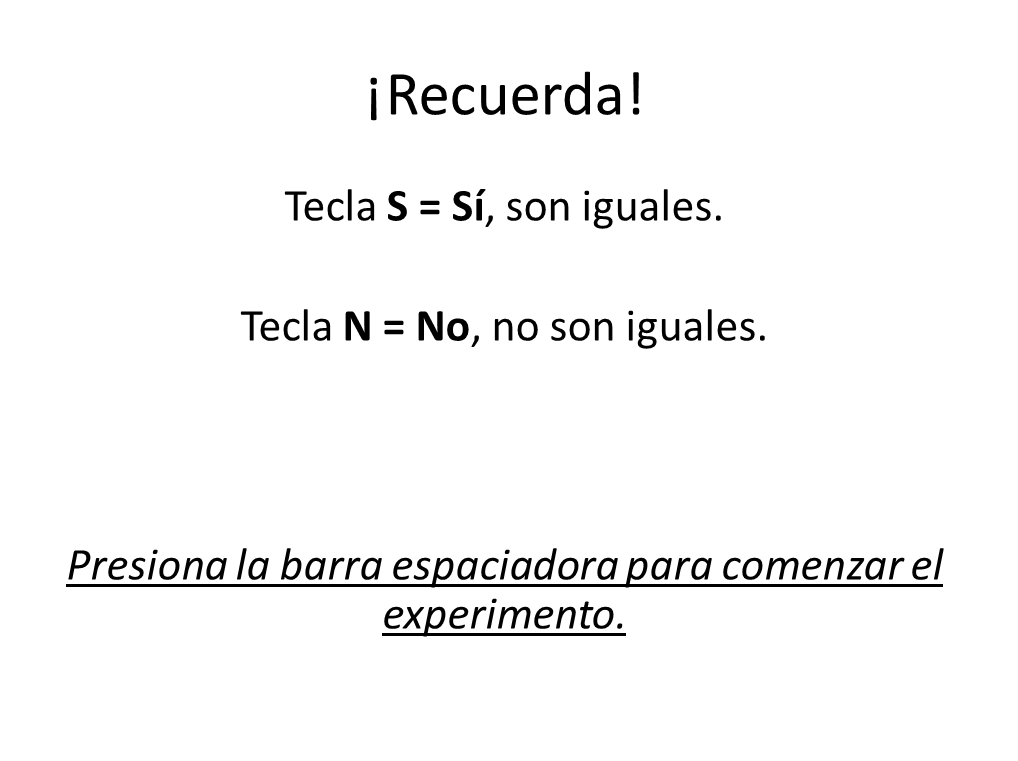
\includegraphics[width=0.75\textwidth]{Figures/Inst_4} 
\decoRule
\caption[Instrucciones finales]{Por último, antes de dar paso al experimento, se mostraba una vez más a los participantes las instrucciones principales del experimento.}
\label{fig:csv}
\end{figure}
